\chapter{Semi-Supervised Learning}\label{ch:SSL}

-\todo{$p$-Lplacian bad for $p$ too small: Numerics and theory}
-\todo{Regularity results $p$-Laplace}
%
\section{Setting}
We are given a finite set $\domain_n\subset \overline{\domain}$ consisting of $n$ points, where $\domain\subset\R^d$ 
is a bounded set. We assume that a subset $\conset_n \subset \domain_n$ is labeled, i.e., we are given a function
$g:\conset_n\to\R$. The semi-supervised learning problem consists in finding an extension of $g$ to the whole set $\domain_n$,
i.e.
%
\begin{gather}\label{eq:SSL}
\begin{gathered}\tag{SSL}
\text{find } u:\domain_n\to\R,\\
\text{such that } u(x) = g(x) \text{ for all } x\in\conset_n.
\end{gathered}
\end{gather}
%
In order to obtain meaningful solutions, one usually incorporates the \emph{smoothness assumption} \cite{} which can be informally stated as follows:
%
\begin{center}
\enquote{\textit{Points that are close together are more likely to share a similar label.}}
\end{center}
%
%
%
\section{The $p$-Laplace Equation}
%
In \cref{sec:SSL_Graphs} we explore concepts that borrow ideas from the theory of partial differential equations, and
in particular the $p$-Laplace equation. In this section we briefly review important ideas and results and provide 
necessary preliminaries for the following sections.
%
\subsection{The $p$-Laplace Equation for $p<\infty$}\label{sec:pLap}
We follow the exposition in \cite{lindqvist2017notes}. Let $\domain\subset\R^d$ be a bounded domain, then 
we consider the $p$-Dirichlet energy for functions $u\in W^{1,p}(\domain)$,
%
\begin{align}\label{eq:DirichletEnergy}
\pDir{}_p(u) := \int_\domain \abs{\Delta_p u}^p \, dx,
\end{align}
%
and the associated variational problem.
%
\begin{problem}{Variational Formulation}{}
For $p\in (1,\infty)$ and $V\subset W^{1,p}(\domain)$ find $u\in V$ such that
%
\begin{align*}
\pDir{}_p(u) \leq \pDir{}_p(v)
\end{align*}
%
for all $v\in V$.
\end{problem}
%
If $u\in V$ is a minimizer of the above problem, then its first variation must vanish, i.e., for all $\phi\in C^\infty_0(\domain)$ 
one has
%
\begin{align}\label{eq:weakLap}
\int_\domain \langle \abs{\Delta_p u}^p \nabla u, \nabla \phi \rangle \, dx = 0.
\end{align}
%
A function $u\in V$ satisfying \cref{eq:weakLap} is called a \emph{weak solution} of the $p$-Laplace equation. In fact, if $u$ 
is smooth enough one has that
%
\begin{align}\label{eq:strongLap}
\Delta_p u := \div(\abs{\Delta_p u}^{p-2} \nabla u) = 0
\end{align}
%
where $\Delta_p$ is called the $p$-Laplacian. For most of our applications we want to prescribe boundary conditions on $\partial \domain$. 
For a given function $g\in W^{1,p}(\domain)$ we therefore consider the set 
$V_g := \{u\in W^{1,p}(\domain): u-g \in W^{1,p}_0(\domain)\}$ for which we have the following result.
%
\begin{theorem}{Existence and Uniqueness}{}
For $p\in (1,\infty)$ and $g\in W^{1,p}(\domain)$ there exists a unique minimizer $u\in V_g$ of the $p$-Dirichlet energy, i.e.,
%
\begin{align*}
\argmin_{u\in V_g} \pDir{}_p(u) = u.
\end{align*}
%
Moreover, $u$ is a weak solution of the $p$-Laplace equation and there exists a function $\tilde{u}\in C(\domain)$ such that
$u = \tilde{u}$ a.e. in $\domain$. If $g\in C(\domain)$ and $\domain$ is sufficiently smooth, then 
$\tilde{u}\vert_{\partial \domain} = g\vert_{\partial \domain}$.
\end{theorem}
%
%
\begin{proof}
The proof can be found in \cite[Thm. 2.16]{lindqvist2017notes}.
\end{proof}
%
%
\paragraph*{Local minimization property}
%
%
\subsection{The $p$-Laplace Equation for $p=\infty$}\label{sec:InfLip}
%
%
This chapter studies the limit $p\to\infty$ of the $p$-Laplace equation. We first recall, that for 
$u\in W^{1,\infty}(\domain)$ we have that
%
\begin{align*}
\lim_{p\to\infty} \pDir{}_p(u)^{1/p} = \esssup_{x\in\domain} \abs{\nabla u(x)} =: \pDir{}_\infty(u),
\end{align*}
%
see \cite{jensen1993uniqueness}. The functional $\pDir{}_\infty$ is weak$^*$-lower semicontinuous over $W^{1,\infty}(\domain)$, 
(see e.g. \cite[Thm. 2.6]{barron2001lower}). In the classical theory developed in \cite{jensen1993uniqueness} one considers the following 
problem.
%
\begin{problem}{}{}
For an open domain $\domain\subset\R^d$ find a function $u\in W^{1,\infty}$ such that
%
\begin{align*}
\norm{\nabla u}_\infty \leq \norm{\nabla v}_\infty \text{ for every } v, \text{s.t. } (u-v)\in W^{1,\infty}_0.
\end{align*}
\end{problem}
%
The above problem becomes more relevant when we additionally impose boundary values $g:\partial\domain\to\R$. Here, 
\cite{jensen1993uniqueness} draws the connection to so-called \emph{Lipschitz extensions}, which are the driving 
concept in this section. We introduce a more general viewpoint on this topic that does not require the notion of a gradient later on. 

\paragraph{The intrinsic metric and the Lipschitz constant.}

As noticed in \cite{jensen1993uniqueness} working with the Lipschitz constant and the sup-norm of the gradient requires a careful 
treatment of the distance measurement. Let $\tilde\domain$ be a set and let $d$ be a semi-metric on $\tilde\Omega$, that is $d$ fulfills 
the requirement of a metric up to triangle inequality. Then we define the Lipschitz constant of a function $u:V\to \R$ on a subset $V\subset \tilde\domain$ as
%
\begin{align*}
\Lip_d(u; V):= \sup_{x,y\in V, x\neq y} \frac{\abs{u(x), u(y)}}{d(x,y)}.
\end{align*}
%
If $d$ denotes the Euclidean distance we use omit the subscript. i.e. $\Lip_d = \Lip$.
For an open domain $\domain\subset\R^d$ and $x,y\in\domain$ we have the inequality
%
\begin{align}\label{eq:LipGrad}
\norm{\nabla u}_\infty\ \abs{x-y} \leq \abs{u(x) - u(y)} \leq \norm{\nabla u}_\infty\ d_\domain(x,y)
\end{align}
%
see, e.g., \cite[Prop9.3, Rem. 7]{brezis2011functional}, where
%
\begin{align*}
d_\domain(x,y) = \inf \left\{
\int_0^1 \abs{\dot{\gamma}(t)} dt : \gamma\in C^1([0,1], \domain)\text{ with } \gamma(0)=x, \gamma(1) =y
\right\}
\end{align*}
%
denotes the \emph{geodesic distance} on $\domain$. If $\domain$ is convex, we have that $d_\domain(x,y) = \abs{x,y}$ for every 
$x,y\in \domain$ and therefore \cref{eq:LipGrad} yields $\Lip(u) = \norm{\nabla u}_\infty$. 

In order to have a geodesic on $\overline{\domain}$ one can simply consider $d_{\overline{\domain}}$, see e.g. \cite{unif}. 
In the classical theory developed in \cite{jensen1993uniqueness} one alternatively considers
%
\begin{align*}
\tilde{d}_{\overline{\domain}}(x,y) := \liminf_{(\tilde x,\tilde y)\to(x,y)} d_\domain(\tilde{x},\tilde{y}).
\end{align*}
%
The differences between these notation are demonstrated in the following example.
%
\begin{example}{}{ex:tube}
For $I = [-\pi, c]\cup [c, \pi]$ with $c=\pi/6$ we consider the domain
%
\begin{align*}
\bigcup_{\theta \in I} B_1\left((\cos(\theta),\sin(\theta)\right)
\end{align*}
%
which is visualized in \cref{fig:tube} and the points $x=(2\, c, 1), y= (2\, c, -1)$. The 
line segment between $x$ and $y$ contains the point $z=(2\, c, 0)$, however $z\notin \domain$. One can show that 
the geodesic has the length $d_\domain(x,y) = 4\, \cos(\pi/6) + \pi \approx 6.606$ which is the length of the dotted path 
in \cref{fig:tube}. However, we observe that 
%
\begin{align*}
\overline{\domain} = \bigcup_{\theta \in I } 
\overline{B_1\left((\cos(\theta),\sin(\theta)\right)}
\end{align*}
%
and in particular $z\in \overline{B_1\left((c,c)\right)}$, therefore $d_{\overline{\domain}}(x,y) = 2$.
\end{example}
%
\begin{figure}
\centering
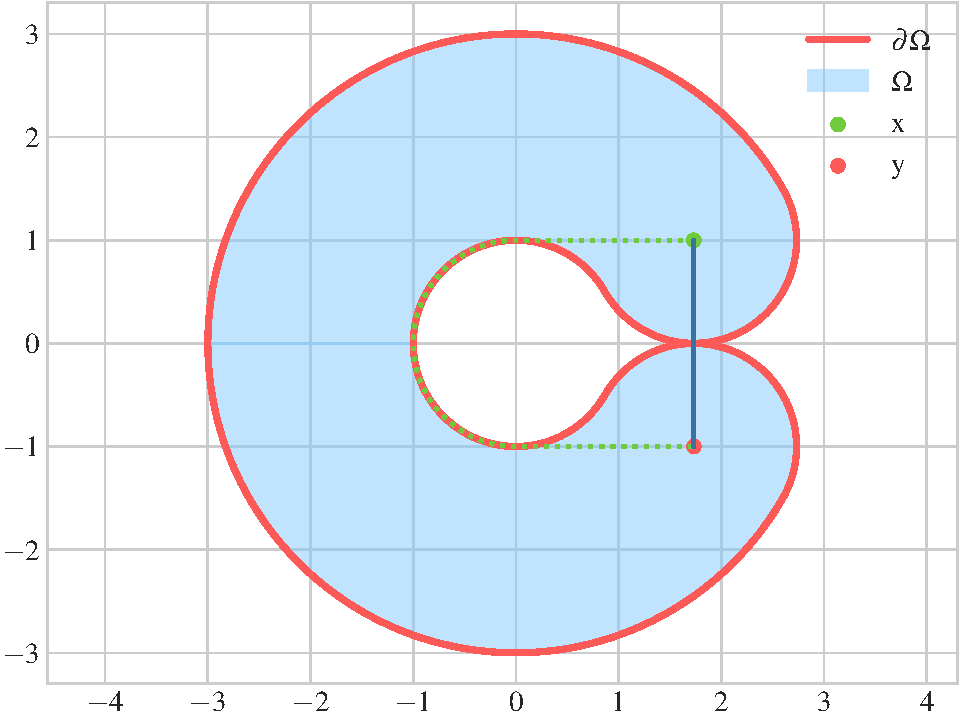
\includegraphics[width=.5\textwidth]{code/domains/tube.pdf}
\caption{The domain in \cref{ex:tube}}\label{fig:tube}
\end{figure}
However, the minimizer is not unique, as demonstrated 
in \cite{jensen1993uniqueness}. 


\todostyle{cool}{color=blue!50!white, bordercolor=white, textcolor=white}
\todo[cool]{Transition}

\paragraph{Lipschitz Extensions}
%
The theory of Lipschitz extensions provides a more general framework. Namely, here we do not assume that $\domain$ is a subset of 
$\R^d$ and rather consider a metric space $(\tilde{\domain},d)$ with $\domain\subset \tilde\domain$. 
%
\begin{remark}{}{}
For applications within this thesis we have that $\domain\subset\R^d$ is an open bounded domain and then consider 
$\tilde\domain:= \closure\domain$, i.e., the closure of $\domain$ within the topology induced by the Euclidean distance. 
In this abstract setting however, we choose to use an abstract space $\tilde\domain$ while still being close notation wise.
\end{remark}
%

%
A result originally due to 
Kierszbraun \cite{Kirszbraun1934} states that for two Hilbert spaces $H_1, H_2$, a subset $U\subset H_1$ and a function $g:\conset\to H_1$ there exists a function $u:H_1\to H_2$ such that 
%
\begin{align*}
u &= g \text{ on } U,\\
\Lip(u; H_1) &= \Lip(g; \conset).
\end{align*}
%
We refer to \cite{Kirszbraun1934} for the original proof and to \cite[Th. 1.31]{Schwartz1969} for a proof of the version as stated above.
In this work we only consider the case $H_2=\R$ which allows for more general assumption on the space $H_1$. We now formulate the Lipschitz extension problem in our setting.
%
\begin{problem}{Lipschitz Extensions}{prob:Lipext}
Let $(\tilde{\domain},d)$ be a metric space and $\conset\subset \tilde{\domain}$ be a bounded subset. For a given Lipschitz function $g:\conset\to\R$ find a Lipschitz function $u:\tilde\domain\to \R$ such that
%
\begin{align*}
\Lip(u; \tilde\domain) = \Lip(g; \conset).
\end{align*}
\end{problem}
%
In this setting one can explicitly construct solutions of the Lipschitz extension task. They are not unique, however one has an upper and a lower bound.
%
\begin{lemma}{}{}
In the setting of \cref{prob:Lipext} we have that the 
%
\begin{itemize}
\item \textbf{Whitney (or maximal) extension:} $\Whit{g}(x) := \inf_{y\in \conset} g(y) + \Lip(g; \conset)\ d(x,y)$ and the
\item \textbf{McShane (or minimal) extension:} $\McS{g}(x) := \sup_{y\in \conset} g(y) - \Lip(g; \conset)\ d(x,y)$
\end{itemize}
%
defined for $x\in\tilde\domain$ are Lipschitz extensions of $g$ to $\tilde\domain$. Moreover, let $u:\tilde\domain\to\R$ be any Lipschitz extension of 
$g$, the we have that
%
\begin{align*}
\McS{g} \leq u \leq \Whit{g}.
\end{align*} 
\end{lemma}
%
\begin{proof}
We refer to \cite{whitney1992analytic} and \cite{mcshane1934extension} for the proofs of the respective result.
\end{proof}
%
The following example demonstrates the above extensions
%
\begin{example}{}{}
This and that a gecko with a hat.
\end{example}
%
As pointed out in \cite{aronsson2004tour} the Whitney and McShane extension do not allow for a comparison principle as the following example 
shows.
%
\begin{example}{}{ex:maxprinc}
Consider the set $\tilde\domain = [-1,1]$ and $\conset=\{-1,0,1\}$ with 
%
\begin{align*}
\color{apple}g_1\bc(x)&:= 0,\\
\color{grape}g_2\bc(x)&:= 1/2 (x- \sign(x)\cdot x),\\
\color{sky}g_3\bc(x)&:= -\color{grape}g_2\bc.
\end{align*}
%
Then we have that $\color{grape}g_2\bc\leq \color{apple}g_1\bc$ on $\conset$ but 
%
\begin{align*}
\color{grape}\Whit{g_2}\bc>\color{apple} \Whit{g_1}\bc \text{ in } (0,1),
\end{align*}
%
see \cref{fig:maxprinc} for a visualization. Analogously, we have that $\color{sky}g_3\bc\geq \color{apple}g_1\bc$ on $\conset$ but 
%
\begin{align*}
\color{sky}\McS{g_3}\bc<\color{apple} \McS{g_1}\bc \text{ in } (0,1).
\end{align*}
\end{example}
%
\begin{figure}
\centering
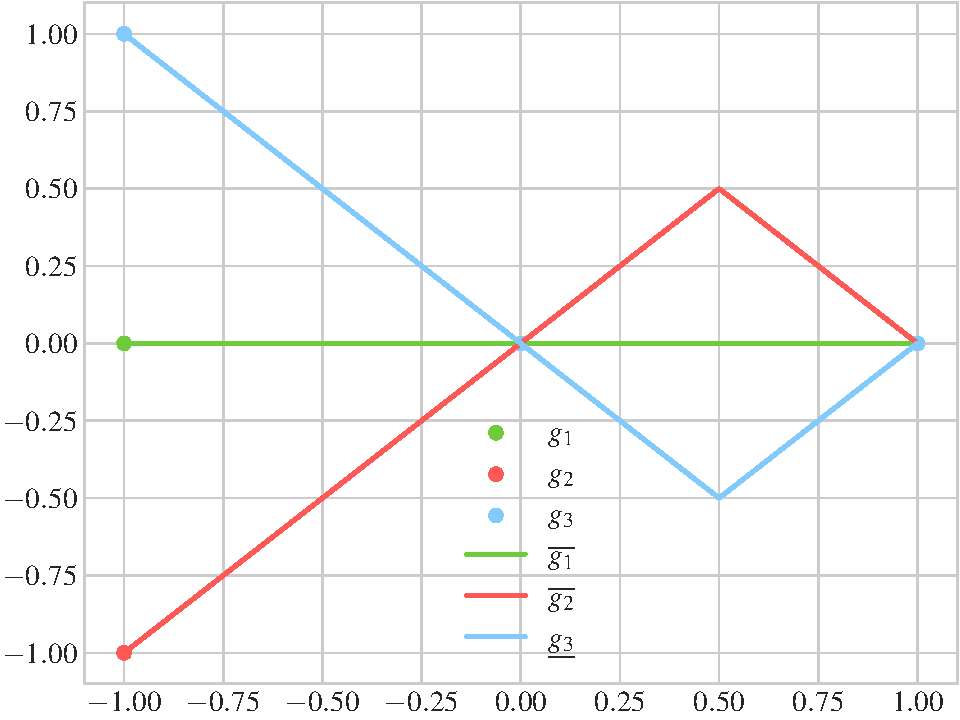
\includegraphics[width=.5\textwidth]{code/lipextcomp/comp.pdf}
\caption{The maximal extension does not admit a comparison principle, as demonstrated in \cref{ex:maxprinc}.}\label{fig:maxprinc}
\end{figure}


\section{Semi-supervised Learning on Graphs}\label{sec:SSL_Graphs}
%
Using the previous insights, we now develop the framework for semi-supervised 
learning on graphs. The key starting point is to introduce weighted graphs, that allow 
us to measure the closeness of points. This concept yields a practical way to 
enforce the smoothness assumption \cref{??}.
%
\begin{definition}{Weighted Graphs}{}
For a finite set $V$ and a weight function $w:V\times V\to\R$, the tuple $(V,w)$ is called a \emph{weighted graph}.
\end{definition}
%
\begin{remark}{}{}
Typically, a graph is defined as a pair $(V,E)$ where $V$ is a finite set and $E$ denotes the set of edges. Here, 
one has two cases:\\
\emph{Undirected graph:} $E=\{ \{x,y\}: \text{there is an edge between } x\in V \text{ and } y\in V\}$, i.e., 
$E\subset 2^V$ and each edge is undirected,\\
%
\emph{Directed graph:} $E=\{ (x,y): \text{there is an edge from } x \text{ to } y\}$, i.e.,
$E\subset V\times V$ and each edge is directed.
%
Additionally, one then considers a weight function $W:E\to\R$ assigning a weight to each edge, and then defines 
the triple $(V,E,W)$ as a weighted graph. However, we note that this information can be represented by a 
weight function $w:V\times V\to\R$. A directed edge set $E\subset V\times V$ can be equivalently expressed by 
a weight function $w:V\times V\to\R$ where $w(x,y)>0$ if and only if $(x,y)\in E$, a weighting $W:E\to\R$ 
naturally transfers to $w$. In the case of an undirected graph, one simply requires the weight function to be symmetric, i.e., 
$w(x,y)=w(y,x)$ for all $x,y\in V$.
%
Furthermore, in the above definition the set $V$ does not enter the definition other than there as a bijection 
$V\to \{1,\ldots,n\}$ for some $n\in \N$. Therefore, a graph could be entirely represented by a weight function 
$w:\{1,\ldots,n\}\times\{1,\ldots,n\}\to\R$. However, since the definition of $w$ will incorporate information
about points $\domain_n\subset\R^d$ we use the notation $(\domain_n, w_n)$ for graphs in the following.
\end{remark}
%
%
In the following we consider functions defined on graphs $\vec{u}:\domain_n\to\R$ for which we employ bold symbols to 
distinguish them from functions in the continuum $u:\domain\to\R$. In particular, the space of graph functions on $\domain_n$ can 
simply be identified with $\R^n$, since 
%
\begin{align*}
\{\vec u:\domain\to\R\} \sim \R^n.
\end{align*}
%
%
\paragraph{Variational Formulation}
While there are various techniques to solve the semi-supervised learning problem \eqref{eq:SSL} \cite{}, 
in this work we 
focus on so-called \emph{Laplacian learning} \cite{belkin2006laplacian}. %
This method had one of its first appearances in 
\cite{zhu2003semi}, where the associated problem was given as
%
\begin{gather}\label{eq:SSL_Laplacian}
\begin{gathered}
\min_{\vec u:\domain_n\to\R} \sum_{x,y\in\domain_n} w_n(x,y)^2 
\left(\vec u(y) - \vec u(x) \right)^2\\
\text{subject to } \vec u(x) = \vec g(x) \text{ for all } x\in\conset_n.
\end{gathered}
\end{gather}
%
A natural extension of this problem is obtained by substituting the target functional by
%
\begin{align*}
J^{w_n,p}(\vec u):= \sum_{x,y\in\domain_n} w_n(x,y)^p \abs{\vec u(y) - \vec u(x)}^p,
\end{align*}
%
which we refer to as the graph $p$-Dirichlet energy. Indeed, we notice structural 
similarities to the $p$-Dirichlet energy in \cref{eq:DirichletEnergy}, replacing the integral by a finite 
sum and derivatives by weighted finite differences
%
\begin{align*}
 w_n(x,y)^p \abs{\vec u(y) - \vec u(x)}^p.
\end{align*}
%
This naturally leads to the following minimization problem.
%
\begin{problem}{Graph Energy Minimization}{prob:vargraph}
Given a weighted graph $(\domain_n, w_n)$ and a labeling function $\vec g:\conset_n\to\R$, for $\conset_n\subset\domain_n$ we consider 
the problem
%
\begin{align*}
\min_{\vec u:\domain_n\to\R} J^{w_n,p}(\vec u) \text{ subject to } \vec u(x) = \vec g(x) \text{ for all } x\in\conset_n.
\end{align*}
\end{problem}
%
Since every function $\vec u:\domain_n\to\R$ can be identified with a vector $\vec u\in\R^n$, the above problem 
is in fact an optimization problem in $\R^n$. Therefore one can prove unique existence of solutions via standard methods.
%
\begin{theorem}{Existence and Uniqueness}{}
\cref{prob:vargraph} admits a unique solution $\vec u:\domain_n\to\R$.
\end{theorem}
%
\begin{proof}
This and that, a gecko with a hat.
\end{proof}
%

\paragraph{Graph Laplacian}
%
In the continuum case one considers the Euler--Lagrange equation for the functional $J^{p}$, which yields the 
$p$-Laplacian, see \cref{sec:pLap}. Analogously, the optimality conditions for the graph $p$-Dirichlet energy $J^{w_n,p}$ yield
%
\begin{align*}
\Delta^{w_n}_p := \sum_{y\in\domain_n} w_n(x,y)^p \abs{\vec u(y) - \vec u(x)}^{p-2} \left( \vec u(y) - \vec u(x) \right) = 0, 
\text{ for all } x\in\domain_n,
\end{align*}
%
where $\Delta^{w_n}_p$ is referred to as the discrete $p$-Laplacian operator. This yields the Graph $p$-Laplacian problem.
%
\begin{problem}{Graph $p$-Laplacian}{prob:graphLaplace}
Given a weighted graph $(\domain_n, w_n)$ and a labeling function $\vec g:\conset_n\to\R$, for $\conset_n\subset\domain_n$ find 
a function $\vec u:\domain_n\to\R$ such that
%
\begin{align*}
\Delta_p^{w_n} \vec u = 0, \text{ in } \domain_n\setminus \conset_n,\\
\vec u = \vec g \text{ on } \conset_n.
\end{align*}
\end{problem}
%
Since the functional $J^{w_n,p}$ has a unique minimizer subject to the constraints given by $\vec g$ and the graph $p$-Laplacian is derived 
via optimality conditions, one expects that the \cref{prob:vargraph} and \cref{prob:graphLaplace} are equivalent. This is formulated in the following 
theorem.
%
\begin{theorem}{Existence and Uniqueness}{}
There exists a unique solution $\vec u:\domain_n\to\R$ to \cref{prob:graphLaplace}, which also is the unique minimizer 
of \cref{prob:vargraph}.
\end{theorem}
%
\begin{proof}
This and that a gecko with a hat.
\end{proof}

\section{Graph Lipschitz Extensions}
%
We now consider the limit $p\to\infty$ of \cref{prob:vargraph} in the graph case. Analogously to \cref{sec:InfLip} we derive
%
\begin{align*}
\lim_{p\to\infty} \left(\GE^{w_n}_p(\vec u)\right)^{1/p}= \max_{x,y\in\domain_n} w_n(x,y) \abs{\vec u(y) - \vec u(x)}=:\GE^{w_n}_\infty(\vec u)
\end{align*}
%
which extends the graph $p$-Laplacian energy to the case $p=\infty$.

\section{Gamma Convergence}
%
\section{Ratio Convergence}
%

